\section{Конструкторская часть}

В данном разделе будут рассмотрены схемы алгоритмов обновления гипертекстового документа с использованием DOM, VDOM и алгоритма согласования. 
Также будут найдены их трудоёмкости и произведено их сравнение на основе полученных результатов.

\subsection{Разработка алгоритмов}

На рисунках \ref{fig:dom-algorithm}--\ref{fig:child-reconciliation-algorithm}, представлены схемы алгоритмов обновления документа с использованием DOM, VDOM, а также алгоритма согласования соответственно.

\clearpage

\begin{figure}[h]
	\centering
	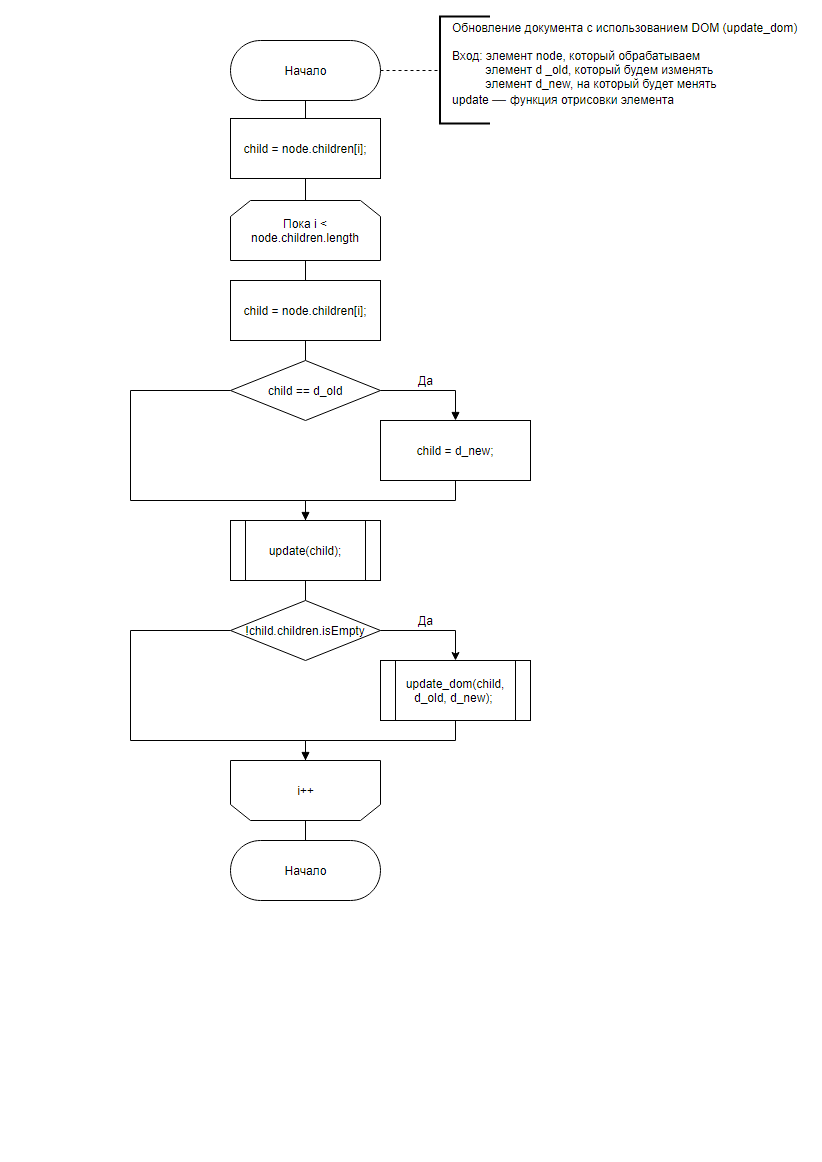
\includegraphics[width=160mm]{img/dom-algorithm.png}
	\caption{Схема алгоритма обновления документа с использованием DOM}
	\label{fig:dom-algorithm}
\end{figure}

\begin{figure}[h]
	\centering
	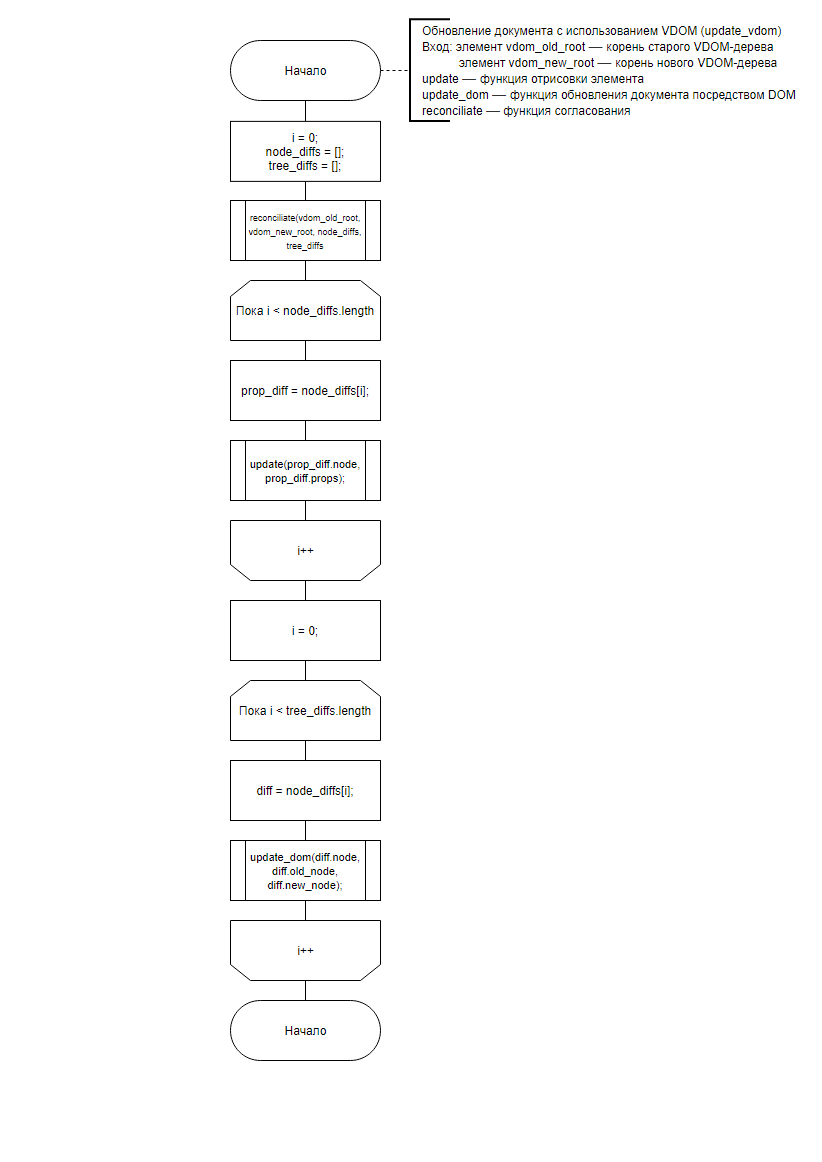
\includegraphics[width=160mm]{img/vdom-algorithm.png}
	\caption{Схема алгоритма обновления документа с использованием VDOM}
	\label{fig:vdom-algorithm}
\end{figure}

\begin{figure}[h]
	\centering
	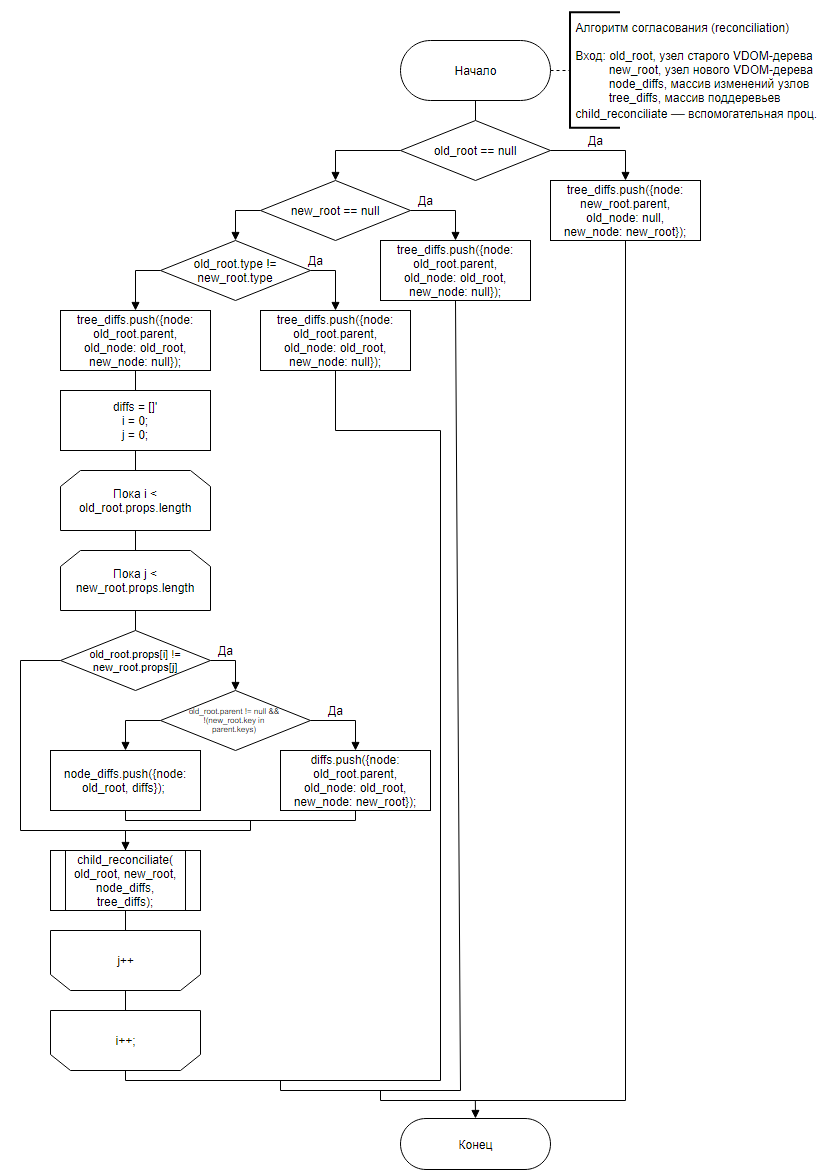
\includegraphics[width=160mm]{img/reconciliation-algorithm.png}
	\caption{Схема алгоритма обновления документа с использованием DOM}
	\label{fig:reconciliation-algorithm}
\end{figure}

\begin{figure}[h]
	\centering
	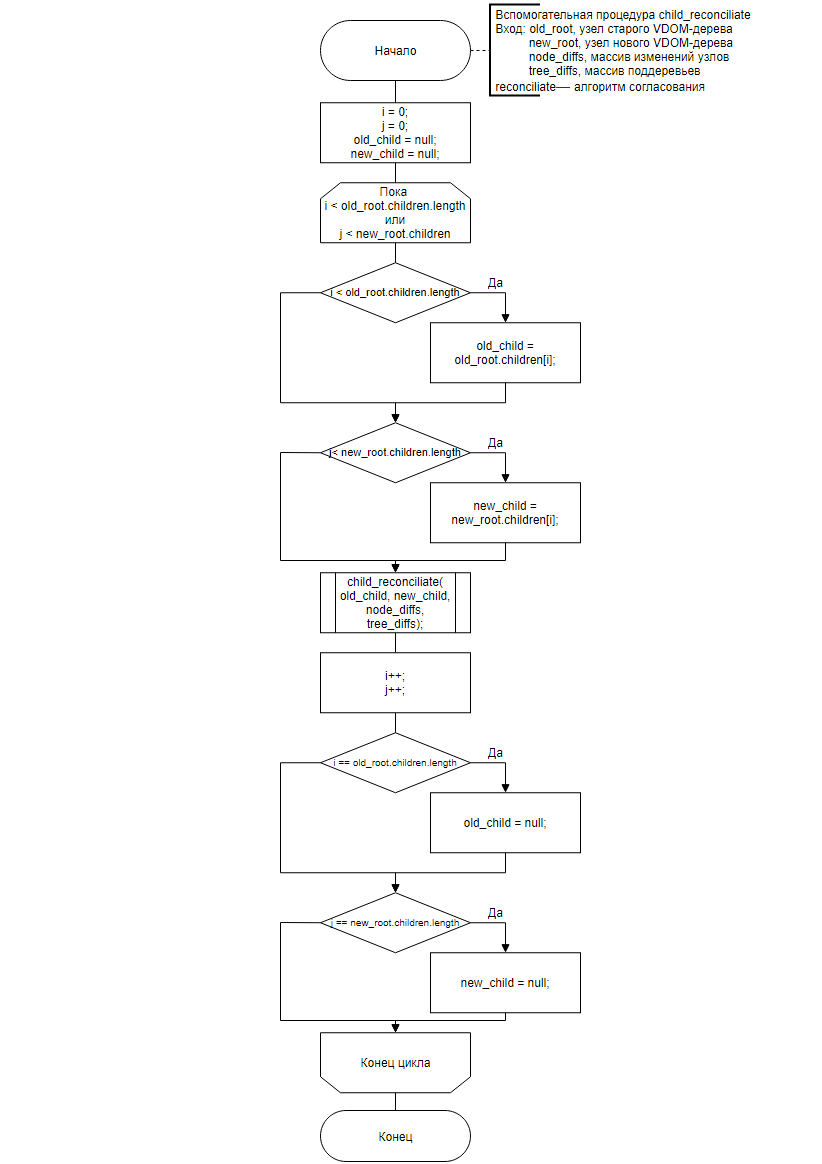
\includegraphics[width=160mm]{img/child-reconciliation-algorithm.png}
	\caption{Схема алгоритма обновления документа с использованием DOM}
	\label{fig:child-reconciliation-algorithm}
\end{figure}

\clearpage

\subsection{Модель вычислений для проведения оценки трудоёмкости}

Введем модель вычислений \cite{model}, которая потребуется для определния трудоемкости каждого отдельно взятого алгоритма сортировки.

\begin{enumerate}[label=\arabic*)]
	\item Операции из списка (\ref{for:operations}) имеют трудоёмкость, равную 1:
	\begin{equation}
		\label{for:operations}
		+, -, /, *, \%, =, +=, -=, *=, ==, !=, <, >, <=, >=, [], ++, {-}-, . 
	\end{equation}
	\item Трудоёмкость оператора выбора \codeword{if условие then A else B} рассчитывается как
	\begin{equation}
		\label{for:if}
		f_{if} = f_{\text{условия}} +
		\begin{cases}
			f_A, & \text{если условие выполняется,}\\
			f_B, & \text{иначе.}
		\end{cases}
	\end{equation}
	\item Трудоёмкость цикла рассчитывается как
	\begin{equation}
		\label{for:cycle}
		f_{for} = f_{\text{инициализации}} + f_{\text{сравнения}} + N(f_{\text{тела}} + f_{\text{инкремент}} + f_{\text{сравнения}}).
	\end{equation}
	\item Трудоёмкость вызова функции равна 0.
\end{enumerate}


\subsection{Трудоёмкость алгоритмов}



\pagebreak